\documentclass[conference]{IEEEtran}
\IEEEoverridecommandlockouts
\usepackage{cite}
\usepackage{balance}
\usepackage{amsmath,amssymb,amsfonts}
\usepackage{graphicx}
\usepackage{textcomp}
\usepackage{xcolor}
\usepackage{booktabs}
\usepackage{array}
\usepackage{tikz}
\usetikzlibrary{positioning,arrows.meta,fit,calc}
\usepackage{algorithm}
\usepackage{algorithmic}
\usepackage[hidelinks]{hyperref}
\newcommand{\PolCases}{16,032}
\newcommand{\PolViol}{0}
\newcommand{\PolAuto}{401}
\newcommand{\PolReview}{3,607}
\newcommand{\PolMonitor}{4,000}
\newcommand{\PolOverride}{8,008}
\newcommand{\PolUnavail}{16}
\newcommand{\PolAutoUnhealthy}{0}
\newcommand{\PolMs}{42}
\newcommand{\EtoECases}{32,032}
\newcommand{\EtoEViolBefore}{2,807}
\newcommand{\EtoEViolAfter}{0}
\newcommand{\EtoEFiredBefore}{9,624}
\newcommand{\EtoEFiredAfter}{6,817}
\newcommand{\DualN}{604}
\newcommand{\DualHold}{69.7}
\newcommand{\DualGap}{64.1}
\newcommand{\DualStraddle}{10.3}
\newcommand{\DualStraddleOnly}{5.6}
\newcommand{\DualEligible}{515}
\newcommand{\DualEligibleHeld}{76.9}
\newcommand{\DualBoth}{453}
\newcommand{\DualBothHeld}{73.7}
\newcommand{\DualMeanGap}{0.167}
\newcommand{\DualMaxGap}{0.347}
\newcommand{\DualRfAuto}{79.5}
\newcommand{\DualXgbAuto}{80.8}
\newcommand{\GuardCtx}{200}
\newcommand{\GuardFacts}{8.1}
\newcommand{\GuardMs}{2.1}
\newcommand{\GuardFalseRej}{0}
\newcommand{\BandCalm}{21}
\newcommand{\BandWatch}{8}
\newcommand{\BandAdmin}{10}
\newcommand{\BandAuto}{161}
\newcommand{\GProbSmallDeployed}{94.0}
\newcommand{\GProbSmallNoscale}{94.0}
\newcommand{\GProbSmallFactsonly}{95.0}
\newcommand{\GProbSmallStrict}{95.0}
\newcommand{\GProbLargeDeployed}{95.5}
\newcommand{\GProbLargeNoscale}{95.5}
\newcommand{\GProbLargeFactsonly}{96.5}
\newcommand{\GProbLargeStrict}{96.5}
\newcommand{\GRainDeployed}{97.0}
\newcommand{\GRainNoscale}{97.0}
\newcommand{\GRainFactsonly}{97.5}
\newcommand{\GRainStrict}{97.5}
\newcommand{\GRiverDeployed}{98.0}
\newcommand{\GRiverNoscale}{98.5}
\newcommand{\GRiverFactsonly}{98.0}
\newcommand{\GRiverStrict}{98.5}
\newcommand{\GCountDeployed}{97.5}
\newcommand{\GCountNoscale}{97.5}
\newcommand{\GCountFactsonly}{98.0}
\newcommand{\GCountStrict}{98.0}
\newcommand{\GEtaDeployed}{94.0}
\newcommand{\GEtaNoscale}{94.0}
\newcommand{\GEtaFactsonly}{95.0}
\newcommand{\GEtaStrict}{95.0}
\newcommand{\GWordsDeployed}{0.0}
\newcommand{\GWordsNoscale}{0.0}
\newcommand{\GWordsFactsonly}{0.0}
\newcommand{\GWordsStrict}{0.0}
\newcommand{\GAllDeployed}{96.0}
\newcommand{\GAllNoscale}{96.1}
\newcommand{\GAllFactsonly}{96.7}
\newcommand{\GAllStrict}{96.8}
\newcommand{\GMissDeployed}{4.0}
\newcommand{\GInjected}{1,200}
\newcommand{\GProbSmallTyped}{97.0}
\newcommand{\GProbLargeTyped}{97.0}
\newcommand{\GRainTyped}{100.0}
\newcommand{\GRiverTyped}{98.5}
\newcommand{\GCountTyped}{100.0}
\newcommand{\GEtaTyped}{100.0}
\newcommand{\GWordsTyped}{81.5}
\newcommand{\GAllTyped}{98.8}
\newcommand{\GTypedFalseRej}{0}
\newcommand{\GTypedMissN}{15}
\newcommand{\GTypedWordMiss}{37}
\newcommand{\DeltaStraddleOnly}{10.3}
\newcommand{\DeltaThirtyHold}{10.9}
\newcommand{\DeltaThirtyBoth}{0.2}
\newcommand{\GMissN}{48}
\newcommand{\GMissFact}{39}
\newcommand{\GMissRule}{8}
\newcommand{\GMissScale}{1}
\newcommand{\GMissEtaFact}{10}
\newcommand{\DeltaZeroBoth}{0.31}
\newcommand{\MissExProb}{87.3}
\newcommand{\MissExEta}{87}
\newcommand{\LiveJudN}{300}
\newcommand{\LiveJudNTwenty}{150}
\newcommand{\LiveJudNOneTwenty}{150}
\newcommand{\LiveN}{300}
\newcommand{\LiveStates}{150}
\newcommand{\LiveUnsup}{109}
\newcommand{\LiveUnsupPct}{36.3}
\newcommand{\LiveTwentyUnsupPct}{33.3}
\newcommand{\LiveOneTwentyUnsupPct}{39.3}
\newcommand{\LiveEta}{106}
\newcommand{\LiveEtaPct}{97}
\newcommand{\LiveOverrides}{4}
\newcommand{\LiveJudgeNone}{23}
\newcommand{\LiveSup}{191}
\newcommand{\LiveDepRec}{89.0}
\newcommand{\LiveDepFpr}{5.8}
\newcommand{\LiveDepPrec}{89.8}
\newcommand{\LiveDepFp}{11}
\newcommand{\LiveTypRec}{93.6}
\newcommand{\LiveTypFpr}{10.5}
\newcommand{\LiveTypPrec}{83.6}
\newcommand{\LiveTypFp}{20}
\newcommand{\LiveJDepRec}{89.0}
\newcommand{\LiveJDepFpr}{5.8}
\newcommand{\LiveJTypRec}{93.6}
\newcommand{\LiveJTypFpr}{10.5}
\newcommand{\LiveJJudRec}{99.1}
\newcommand{\LiveJJudFpr}{14.1}
\newcommand{\LiveJUnsup}{109}
\newcommand{\LiveJJudMiss}{1}
\newcommand{\LiveDepMiss}{12}
\newcommand{\LiveDepMissWords}{5}
\newcommand{\LiveDepMissClock}{5}
\newcommand{\LiveTypFpN}{20}
\newcommand{\LiveOverclaim}{43}
\newcommand{\LiveOverclaimPct}{14}
\newcommand{\LiveDigitEtaCaught}{97}
\newcommand{\JudgeInjStates}{40}
\newcommand{\JudgeInjItems}{320}
\newcommand{\JudgeFalseRej}{0.0}
\newcommand{\JudgeFalseRejN}{0}
\newcommand{\JudgeInjNum}{97.1}
\newcommand{\JudgeProbSmallMiss}{15}
\newcommand{\JudgeInjWords}{90.0}
\newcommand{\DepInjNumSub}{96.7}
\newcommand{\TypInjNumSub}{99.2}
\newcommand{\JudgeModel}{Qwen3 (27B)}
\newcommand{\CalTest}{910}
\newcommand{\CalTrain}{3638}
\newcommand{\CalPos}{35.8}
\newcommand{\EceRf}{0.044}
\newcommand{\EceCalRf}{0.031}
\newcommand{\BrierRf}{0.163}
\newcommand{\MeanPRf}{0.379}
\newcommand{\EceXgb}{0.108}
\newcommand{\EceCalXgb}{0.018}
\newcommand{\BrierXgb}{0.182}
\newcommand{\MeanPXgb}{0.378}
\newcommand{\CalGapMean}{0.101}
\newcommand{\DeltaCv}{0.28}
\newcommand{\GateDepHold}{26.9}
\newcommand{\GateDepBoth}{29.1}
\newcommand{\GateDepErrHeld}{37.1}
\newcommand{\GateDepErrRel}{20.3}
\newcommand{\GateCvHold}{9.1}
\newcommand{\GateCvBoth}{2.2}
\newcommand{\GateCvErrHeld}{48.2}
\newcommand{\GateCvErrRel}{22.5}
\newcommand{\GateStHold}{7.6}
\newcommand{\GateStBoth}{0.0}
\newcommand{\GateStErrHeld}{52.2}
\newcommand{\GateStErrRel}{22.6}
\newcommand{\GateCalHold}{10.5}
\newcommand{\GateCalBoth}{7.0}
\newcommand{\GateDepErrRatio}{1.8}
\newcommand{\GateStErrRatio}{2.3}
\newcommand{\XgbHighConf}{0.84}
\newcommand{\XgbHighFreq}{0.67}
\newcommand{\DevDepRec}{89.0}
\newcommand{\DevDepFpr}{5.8}
\newcommand{\HoDepRec}{96.1}
\newcommand{\HoDepFpr}{7.1}
\newcommand{\HoDepFp}{4}
\newcommand{\HoDepMiss}{3}
\newcommand{\DevTypRec}{93.6}
\newcommand{\DevTypFpr}{10.5}
\newcommand{\HoTypRec}{100.0}
\newcommand{\HoTypFpr}{17.9}
\newcommand{\HoTypFp}{10}
\newcommand{\HoTypMiss}{0}
\newcommand{\DevVtwoRec}{100.0}
\newcommand{\DevVtwoFpr}{0.0}
\newcommand{\HoVtwoRec}{98.7}
\newcommand{\HoVtwoFpr}{12.5}
\newcommand{\HoVtwoFp}{7}
\newcommand{\HoVtwoMiss}{1}
\newcommand{\HoN}{132}
\newcommand{\HoStates}{150}
\newcommand{\HoUnsup}{76}
\newcommand{\HoUnsupPct}{57.6}
\newcommand{\HoParseFail}{18}
\newcommand{\HoCountPct}{67}
\newcommand{\HoOverrides}{8}
\newcommand{\VtwoUs}{371}
\newcommand{\VtwoInjGround}{0.0}
\newcommand{\VtwoInjNum}{98.8}
\newcommand{\VtwoInjWords}{81.5}
\newcommand{\ErrOssEtaMin}{32}
\newcommand{\ErrOssEtaMax}{39}
\newcommand{\ErrAllamEta}{4.5}
\newcommand{\ErrAllamQty}{39}
\newcommand{\ErrAllamProb}{16}
\newcommand{\JudgeCiMax}{14}
\newcommand{\JudFailN}{23}
\newcommand{\JudFailSup}{15}
\newcommand{\JudFailUnsup}{8}
\newcommand{\JudAnsN}{277}
\newcommand{\JudAnsRec}{99.0}
\newcommand{\JudAnsFpr}{6.8}
\newcommand{\JudAnsMiss}{1}
\newcommand{\JudAnsDepFpr}{5.1}
\newcommand{\JudAnsTypFpr}{10.2}
\newcommand{\JudAnsDepRec}{88.1}
\newcommand{\JudAnsTypRec}{93.1}
\newcommand{\JudAllCiLo}{95}
\newcommand{\JudAllCiHi}{100}
\newcommand{\McVtwoRecOnly}{3}
\newcommand{\McDepRecOnly}{1}
\newcommand{\McVtwoRecP}{0.62}
\newcommand{\McVtwoFpOnly}{3}
\newcommand{\McVtwoFpP}{0.25}
\newcommand{\McDevTypRecP}{0.062}
\newcommand{\McDevTypFpP}{0.004}
\newcommand{\FbTwenty}{38.7}
\newcommand{\FbOneTwenty}{33.3}
\newcommand{\FbAllam}{63.3}
\newcommand{\AllamFailAuto}{18}
\newcommand{\AllamAutoCalls}{123}
\newcommand{\AllamOtherCalls}{27}
\newcommand{\NsDevRec}{89.0}
\newcommand{\NsDevFpr}{6.3}
\newcommand{\NsHoRec}{97.4}
\newcommand{\NsHoFpr}{12.5}
\newcommand{\PoDevUnsup}{113}
\newcommand{\PoHoUnsup}{84}
\newcommand{\PoDevDepRec}{88.5}
\newcommand{\PoDevDepFpr}{4.3}
\newcommand{\PoDevTypRec}{93.8}
\newcommand{\PoDevTypFpr}{8.6}
\newcommand{\PoDevVtwoRec}{96.5}
\newcommand{\PoDevVtwoFpr}{0.0}
\newcommand{\PoHoDepRec}{91.7}
\newcommand{\PoHoDepFpr}{0.0}
\newcommand{\PoHoTypRec}{98.8}
\newcommand{\PoHoTypFpr}{6.2}
\newcommand{\PoHoVtwoRec}{97.6}
\newcommand{\PoHoVtwoFpr}{0.0}
\newcommand{\OcDev}{43}
\newcommand{\OcDevPct}{14.3}
\newcommand{\OcDevPassDep}{27}
\newcommand{\OcDevPassTyp}{24}
\newcommand{\OcDevPassVtwo}{23}
\newcommand{\OcDevPassJud}{20}
\newcommand{\OcDevPassDepPct}{63}
\newcommand{\OcDevPassJudPct}{47}
\newcommand{\OcHo}{8}
\newcommand{\EtoEHigh}{401}
\newcommand{\SweepAuto}{488}
\newcommand{\SweepAutoRel}{119}
\newcommand{\SweepN}{604}
\newcommand{\GtErrN}{226}
\newcommand{\GtDepCaught}{91}
\newcommand{\GtDepRecall}{40.3}
\newcommand{\GtStCaught}{36}
\newcommand{\GtStRecall}{15.9}
\newcommand{\GtStHolds}{69}
\newcommand{\GtDepHolds}{245}
\newcommand{\GtMore}{55}
\newcommand{\GtMoreLo}{42}
\newcommand{\GtMoreHi}{69}
\newcommand{\GtCalT}{0.18}
\newcommand{\GtCostDepFive}{62.9}
\newcommand{\GtCostCalFive}{50.0}
\newcommand{\GtCostDepOne}{20.2}
\newcommand{\GtCostNoneOne}{24.8}
\newcommand{\ClsEvents}{4,548}
\newcommand{\ClsGauges}{155}
\newcommand{\ClsNum}{55}
\newcommand{\ClsCat}{4}
\newcommand{\ClsPos}{35.8}
\newcommand{\ClsAucRf}{0.818}
\newcommand{\ClsAucXgb}{0.806}
\newcommand{\ClsAccXgb}{75.2}
\newcommand{\ClsAccRf}{75.5}
\newcommand{\ClsTOneP}{188}
\newcommand{\SweepAboveP}{37}
\newcommand{\VarN}{233}
\newcommand{\VarStates}{120}
\newcommand{\VarBaseN}{100}
\newcommand{\VarBaseUnsup}{28.0}
\newcommand{\VarBaseEta}{26.0}
\newcommand{\VarBaseFb}{26.0}
\newcommand{\VarBaseClaim}{8.0}
\newcommand{\VarBaseTok}{634}
\newcommand{\VarBaseWords}{64}
\newcommand{\VarBaseParsed}{100}
\newcommand{\VarNoetaUnsup}{3.4}
\newcommand{\VarNoetaEta}{0.4}
\newcommand{\VarNoetaFb}{2.6}
\newcommand{\VarNoetaClaim}{17.6}
\newcommand{\VarNoetaTok}{664}
\newcommand{\VarNoetaWords}{67}
\newcommand{\VarNoetaParsed}{233}
\newcommand{\VarSlotsUnsup}{1.7}
\newcommand{\VarSlotsEta}{0.4}
\newcommand{\VarSlotsFb}{0.0}
\newcommand{\VarSlotsClaim}{5.1}
\newcommand{\VarSlotsTok}{734}
\newcommand{\VarSlotsWords}{57}
\newcommand{\VarSlotsParsed}{234}
\newcommand{\VarSlotsViol}{2.1}
\newcommand{\VarSlotsFbSlot}{2.1}
\newcommand{\VarSlotsResid}{1}
\newcommand{\VarOldProtoUnsup}{37.7}
\newcommand{\DesignText}{Re-run on the same day, the production prompt still produced an unsupported number in 28.0\% of replies (the script's label for the original run: 37.7\%). One added line forbidding arrival times lowered this to 3.4\% and arrival times from 26.0\% to 0.4\% of replies, at a cost of 30 prompt and output tokens per call. The slots-only prompt left a digit or number word in 2.1\% of replies, which therefore fall back to the template (2.1\% of calls in all). Of the replies that passed this check, one still contained an unsupported number after rendering. Its replies were 57 words long against 64 and used 734 tokens per call against 634; whether the placeholder style reads as well on a radio net is a question for officers.}
\newcommand{\SlotsAbstract}{left a digit or number word in 2.1\% of replies, which then fall back to the template; 1 replies that passed still did.}
\newcommand{\ConclusionDesign}{Forbidding arrival times in the prompt cut unsupported replies from 28.0\% to 3.4\%, and a narrator that writes only placeholders left 1 unsupported number in 234 replies, at the price of 2.1\% template fallbacks.}
\newcommand{\ClaimText}{The frozen claim check flagged 8.0\%, 17.6\% and 5.1\% of the replies to the three prompts of Table~\ref{tab:design}, which it had never seen.}


\begin{document}

\title{Rules Decide, Language Models Narrate:\\
Fail-Closed Numeric Grounding of LLM Narration\\
in a Flood-Response Pipeline}

%<AUTHORS>
\author{
\IEEEauthorblockN{Nandhakumar T}
\IEEEauthorblockA{\textit{Department of Information Technology}\\
\textit{Sona College of Technology}\\
Salem, Tamil Nadu, India\\
nandhakumartm93@gmail.com}
\and
\IEEEauthorblockN{Balakarthikeyan B S}
\IEEEauthorblockA{\textit{Department of Artificial Intelligence and Data Science}\\
\textit{Sona College of Technology}\\
Salem, Tamil Nadu, India\\
balasan2626@gmail.com}
\and
\IEEEauthorblockN{Gowthaman J}
\IEEEauthorblockA{\textit{Department of Artificial Intelligence and Data Science}\\
\textit{Sona College of Technology}\\
Salem, Tamil Nadu, India\\
gowthamanjanadhran@gmail.com}
\and
\IEEEauthorblockN{Abhishek S}
\IEEEauthorblockA{\textit{Department of Artificial Intelligence and Data Science}\\
\textit{Sona College of Technology}\\
Salem, Tamil Nadu, India\\
abisheksengodan18@gmail.com}
}
%</AUTHORS>

\maketitle

\begin{abstract}
Large language models (LLMs) are proposed as the voice of emergency-management software, but they can state numbers that are not in the data. We study a flood-response pipeline in which a deterministic policy chooses every action and an LLM only narrates, behind three fail-closed checks: a health-gated policy, a disagreement gate between two classifiers and a numeric guard that replaces a message containing an unsupported number by a template. We evaluate the checks on the deployed code. A composed check of the path from policy to dispatch showed that dispatch ignored the policy whenever a health check failed at high flood probability (\EtoEViolBefore{} grid cases); a one-line fix removed every such case. Of \LiveN{} replies from two open-weight models, \LiveUnsupPct\% contained an unsupported number, \LiveEta{} of \LiveUnsup{} of them invented arrival times. The deployed guard caught \LiveDepRec\% and a slot-typed guard \LiveTypRec\%. A narrator that writes placeholders and leaves every number to the program, tested live, \SlotsAbstract{} A revised guard frozen before a third model was queried was not significantly better than the deployed guard on that model. No numeric guard sees qualitative over-claims such as ``flood confirmed'', which \OcDevPct\% of replies made, so our grounding claim covers numbers only; a frozen check on assertion words flags such claims. The gate held \GateDepHold\% of held-out cases and caught \GtDepRecall\% of the policy model's errors. All rates are specific to our prompt, models and states.
\end{abstract}

\begin{IEEEkeywords}
large language models, hallucination, fail-safe design, runtime verification, flood response
\end{IEEEkeywords}

\section{Introduction}
During a flood, an emergency operations centre runs on short spoken messages: the river is at this level, the forecast says this, send a team there. Software that supports the centre is increasingly asked to \emph{speak}, and LLMs make this easy. They also produce confident statements that their input does not support \cite{Ji2023}. On an operations net a wrong number, or a wrong claim that a flood has started, can trigger or cancel an evacuation.

Agentic systems let the model plan and call tools \cite{Yao2023,Wu2024}. For a safety-critical setting we take the opposite position: decisions are made by small deterministic rules that can be checked exhaustively, and the LLM only turns their state into radio traffic. This follows the view that the level of automation should be chosen per function and per risk \cite{Parasuraman2000} and that safety is a property of the control structure rather than of one component \cite{Leveson2011}. The design is close to a classical alerting pipeline, in which a rule fills a structured message such as a Common Alerting Protocol (CAP) alert \cite{CAP2010}; what is new is a free-text narrator inside it. Two questions follow. Does the verified decision govern what the system does? And how often does the narrator misstate the state, and which design or check prevents it?

We answer both on an open flood decision-support prototype for the Delhi Yamuna corridor:
\begin{enumerate}
\item A composed check of the path from policy to dispatch, with its equivalence classes, which found that dispatch bypassed the policy and confirmed the fix.
\item A measurement of numeric grounding on \LiveN{} live replies of two open-weight LLMs and on injected errors, comparing the deployed guard, a slot-typed guard, an LLM judge and two prompt designs, including one in which the LLM writes no number at all.
\item A held-out test of a revised guard on a third model family, frozen by hash before its replies were read, with paired tests, and a frozen check for qualitative over-claims.
\item A held-out study of the disagreement gate that reports the share of errors it catches and its cost against a calibrated single model.
\end{enumerate}
A companion paper on the whole decision chain reuses the dispatch result and the guard results on the development replies; this paper reports the full guard study, the prompt designs and the gate.

\section{Related Work}
\textit{LLM agents} interleave reasoning with actions \cite{Yao2023} and cooperate in conversations \cite{Wu2024}; surveys describe them as memory, planner and action interface around a model \cite{WangL2024}.

\textit{Hallucination detection and guardrails.} Generated text departs from its source in many ways \cite{Ji2023}. Retrieval grounds generation in documents \cite{Lewis2020}; post-hoc checkers decompose text into atomic claims \cite{Min2023}, sample the model several times \cite{Manakul2023}, let the model verify itself \cite{Dhuliawala2024} or ask another model to judge \cite{Zheng2023}. NeMo Guardrails programs dialogue rails and checks facts with a further model call \cite{Rebedea2023}, which is the setting of our LLM-judge baseline; runtime verification checks outputs against expert specifications \cite{Zhang2025}, and runtime enforcement blocks unsafe agent actions \cite{WangH2026}. Our facts are a handful of numbers in a known state, so a deterministic, typed check is possible, and so is a design in which the model writes no numbers.

\textit{Safe automation.} Shields block unsafe actions of learned controllers \cite{Alshiekh2018}, and ensembles estimate uncertainty \cite{Lakshminarayanan2017}. We use disagreement between two classifiers as a hold signal.

\textit{Research gap.} We found no study that measures, on an emergency system's deployed code, whether a verified decision governs actuation and how often live LLM narration misstates numeric state, comparing deterministic checks, a model judge and a numbers-free narrator.

\section{Architecture}
\label{sec:arch}
Fig.~\ref{fig:arch} shows the system. A FastAPI backend runs one pipeline per tick, in live mode (Open-Meteo weather and river data) or in simulation mode (a digital twin of the corridor). The code calls its eleven components agents (weather, dam, flood risk, traffic, shelter, evacuation, rescue, ambulance, disaster team, administrator and a monitor of sudden changes). Ten of them inform, rank, propose or narrate; only the policy (\ref{eq:policy}) decides, and dispatch executes only what it allowed. The system is therefore a rule-based pipeline with an LLM narrator, and we use the code's names only to identify components. Every event goes to a MongoDB log and a WebSocket stream. Algorithm~\ref{alg:tick} gives one tick; narration runs last, after the decision is logged, so a narration failure can delay a radio message but cannot change a decision.

\begin{algorithm}[t]
\caption{One pipeline tick (after the fix)}
\label{alg:tick}
\begin{algorithmic}[1]
\small
\STATE read observations; weather and dam components emit updates
\STATE $p_{\mathrm{RF}},p_{\mathrm{XGB}},p \leftarrow$ classifiers; $H\leftarrow$ (\ref{eq:dual})
\STATE $(h_d,h_m,h_s)\leftarrow$ health checks; $a\leftarrow\pi(p,\mathbf{h},o)$ by (\ref{eq:policy})
\STATE \textbf{if} $H$ \AND \NOT $o$ \textbf{then} $a\leftarrow\textsc{review}$ and log the hold reason
\STATE \textbf{if} $a\neq\textsc{monitor}$ \textbf{then} rank roads, shelters, routes
\STATE \textbf{if} $a\in\{\textsc{auto},\textsc{override}\}$ \AND band$(p)=$ auto \textbf{then} dispatch
\STATE $T\leftarrow$ LLM turns for band$(p)$; \textbf{if} \NOT $\Gamma(T)$ \textbf{then} $T\leftarrow$ template
\STATE broadcast state, decision and $T$
\end{algorithmic}
\end{algorithm}

\begin{figure}[t]
\centering
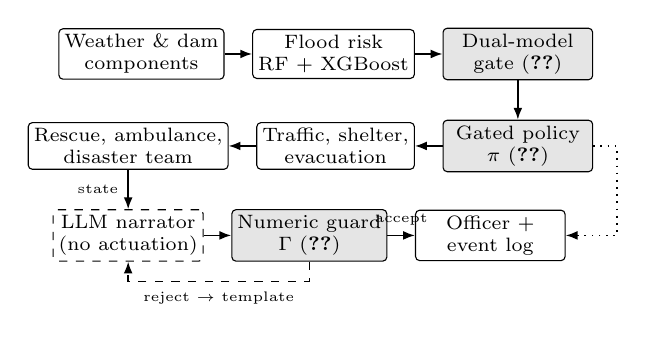
\begin{tikzpicture}[
  font=\scriptsize,
  box/.style={draw, rounded corners=1.5pt, align=center, minimum width=1.9cm, minimum height=0.58cm, inner sep=2pt},
  gate/.style={box, fill=gray!20},
  llm/.style={box, dashed},
  arr/.style={-{Latex[length=1.5mm]}, semithick}]
\node[box] (wx) {Weather \& dam\\components};
\node[box, right=0.35cm of wx] (fr) {Flood risk\\RF + XGBoost};
\node[gate, right=0.35cm of fr] (dual) {Dual-model\\gate (\ref{eq:dual})};
\node[gate, below=0.5cm of dual] (pol) {Gated policy\\$\pi$ (\ref{eq:policy})};
\node[box, left=0.35cm of pol] (ops) {Traffic, shelter,\\evacuation};
\node[box, left=0.35cm of ops] (res) {Rescue, ambulance,\\disaster team};
\node[llm, below=0.5cm of res] (llm) {LLM narrator\\(no actuation)};
\node[gate, right=0.35cm of llm] (guard) {Numeric guard\\$\Gamma$ (\ref{eq:guard})};
\node[box, right=0.35cm of guard] (hum) {Officer +\\event log};
\draw[arr] (wx) -- (fr);
\draw[arr] (fr) -- (dual);
\draw[arr] (dual) -- (pol);
\draw[arr] (pol) -- (ops);
\draw[arr] (ops) -- (res);
\draw[arr] (res) -- node[left, font=\tiny]{state} (llm);
\draw[arr] (llm) -- (guard);
\draw[arr] (guard) -- node[above, font=\tiny]{accept} (hum);
\draw[arr, dashed] (guard.south) -- ++(0,-0.25) -| node[pos=0.25, below, font=\tiny]{reject $\rightarrow$ template} (llm.south);
\draw[arr, dotted] (pol.east) -- ++(0.3,0) |- (hum.east);
\end{tikzpicture}
\caption{Pipeline. Shaded blocks can only hold, downgrade or reject; none can trigger an action. The LLM (dashed) receives the shared state and has no actuation rights. The dotted link carries every policy decision and its reason to the officer.}
\label{fig:arch}
\end{figure}

\subsection{Decision Policy}
The flood-risk component receives a flood probability $p$ and three health flags: $h_d$ (weather and river data available), $h_m$ (model loaded and returned a value) and $h_s$ (database connected). An operator can set an override $o$, and a flag $A$ enables automation. With $\tau_m=0.50$ and $\tau_a=0.60$, served from one configuration module,
\begin{equation}
\pi(p,\mathbf{h},o)=
\begin{cases}
\textsc{unavailable} & p \text{ undefined}\\
\textsc{override} & o\\
\textsc{monitor} & p<\tau_m\\
\textsc{auto} & p\ge\tau_a \wedge h_d\wedge h_m\wedge h_s\wedge A\\
\textsc{review} & \text{otherwise.}
\end{cases}
\label{eq:policy}
\end{equation}

\subsection{Classifiers and the Disagreement Gate}
Two classifiers score the same inputs: a Random Forest \cite{Breiman2001} and an XGBoost model \cite{Chen2016}, the latter supplying $p$. Both were trained on the INDOFLOODS catalogue (\ClsEvents{} flood events at \ClsGauges{} gauges) to predict whether an event is \emph{severe}; the label is the catalogue's flood type, and \ClsPos\% of events are severe. Their \ClsNum{} numeric and \ClsCat{} categorical inputs are rainfall over the last 1 to 10 days with engineered ratios, the season, catchment attributes and a gauge prior. A stratified random 80/20 split of events gave a held-out ROC-AUC of \ClsAucRf{} (RF) and \ClsAucXgb{} (XGBoost) and an accuracy at $\tau_a$ of \ClsAccRf\% and \ClsAccXgb\%. The ``flood probability'' that the system displays is therefore the probability that a flood event at the corridor's gauge would be severe. Automatic dispatch is held when
\begin{multline}
H=\big[\,|p_{\mathrm{RF}}-p_{\mathrm{XGB}}|\ge\delta\,\big]\\
\vee\ \big[\min(p_{\mathrm{RF}},p_{\mathrm{XGB}})<\tau_a\le\max(p_{\mathrm{RF}},p_{\mathrm{XGB}})\big],
\label{eq:dual}
\end{multline}
with $\delta=0.15$; the second, \emph{straddle} term flags models on opposite sides of the threshold.

\subsection{LLM Narration and the Numeric Guards}
Agent conversations are generated by an LLM through an external API. The band follows $p$ (calm below 0.40, watch below 0.50, administrator review below 0.60, automated response above) and sets who speaks and the tone; the action is still set by $\pi$. The prompt lists the current facts (probabilities, rainfall, river level, barrage stage, time and place), states the band's rule and tells the model to use only those numbers. The rule of the automated band reads ``Above 60\%: flood occurred'', and the template that replaces a rejected reply begins ``Flood has occurred''; Section~\ref{sec:claims} returns to this wording.

Let $\mathcal{N}(s)$ be the decimal numbers in a string $s$ and $F$ the prompt text up to the recent-history block. With $\tilde F=\{f,100f,f/100: f\in\mathcal{N}(F)\}$, the deployed guard accepts turns $T$ when
\begin{equation}
\Gamma(T)=\bigwedge_{t\in T}\ \bigwedge_{n\in\mathcal{N}(t)}\ \exists f\in\tilde F:\ |n-f|\le \tfrac12 10^{-d(n)},
\label{eq:guard}
\end{equation}
where $d(n)$ is the number of decimals written in $n$, so honest rounding passes. The guard is untyped: a number written as a word is invisible to it, and a value drawn uniformly from an integer range $[a,b]$ passes with probability
\begin{equation}
P_{\mathrm{miss}}\approx |\{\lfloor f\rceil : f\in\tilde F\}\cap[a,b]|\,/\,(b-a+1).
\label{eq:miss}
\end{equation}

\textit{Slot-typed guard.} $\Gamma_{\mathrm{T}}$ reads facts from the structured state and binds each number to a quantity before checking it: number words become digits, clock times must equal the current time, a number with ``\%'' must match a model probability or a threshold of the band, one with ``mm'' the rainfall and one with ``m'' a water level. An unbound number is rejected. A revised version, $\Gamma_{\mathrm{T}}^{(2)}$, adds procedural numbers (reporting intervals, deadlines given as orders), rejects every arrival time and binds a value without a unit to the quantity named just before it.

\textit{Slots-only narrator.} As an alternative to checking numbers, the prompt can forbid them: the model writes no digit or number word and refers to facts by placeholders (\{probability\}, \{rain\_mm\}, \{river\_m\}, \{barrage\_m\}, \{time\}, \{threshold\}, \{places\}), which the program fills from the state. A reply that still contains a digit, a number word or an unknown placeholder is replaced by the template.

\section{Evaluation Setup}
\textit{Policy and dispatch path.} We evaluated (\ref{eq:policy}) on $p\in\{0,0.001,\dots,1\}$ plus an undefined value, all eight health combinations and both override states ($1{,}002\times8\times2=$ \PolCases{} cases), against five properties (\textsc{auto} only if every check passes and $p\ge\tau_a$; undefined $p$ gives \textsc{unavailable}; $p<\tau_m$ without override gives \textsc{monitor}; $p\ge\tau_a$ with a failed check gives \textsc{review}; monotone in $p$ when healthy). We then extracted the dispatch decision into a pure function and checked the composed path (policy, hold, dispatch) over every defined probability, health combination, hold and override ($1{,}001\times8\times2\times2=$ \EtoECases{} cases) for the property that teams are dispatched only when every check passes and the models agree, or an operator overrides. Because $p$ enters both functions only through comparisons with 0.40, 0.50 and 0.60, all of which lie on the grid, the grid contains every equivalence class, so each check is a proof for the extracted functions, not a sample.

\textit{Live replies.} For \LiveStates{} seeded states (rainfall 5--250~mm in a monsoon month, both model probabilities from the deployed classifiers, river 200.0--208.5~m, barrage 199.0--206.0~m) we sent the production prompt to gpt-oss-20b and gpt-oss-120b on Groq at temperature 0.85 without fallback (\LiveN{} replies, all parsed), and stored the verdict of each check. Reference labels follow a written protocol. A number is \emph{supported} if it states a state value for the quantity it describes (honest rounding allowed) or quotes a band threshold; \emph{procedural} numbers (reporting intervals, unit labels, the count of named places, band ranges, deadlines given as orders) are ignored; anything else, including any arrival time, is \emph{unsupported}. The protocol was applied by a script; replies on which it disagreed with any checker were then read, and \LiveOverrides{} labels were changed, all to ``procedural''. Because this reading saw the checkers' verdicts, we also report every result under the script's labels alone.

\textit{Prompt designs.} For the first \VarStates{} of these states and the same models we ran two further prompts on one day (the run was stopped there to limit API use): the production prompt plus one line forbidding arrival times, and the slots-only prompt (\VarN{} calls each), plus the unchanged production prompt on the first 50 states (\VarBaseN{} calls) to check for drift. These replies were labelled by the script only.

\textit{LLM judge.} Qwen3 (27B), a family different from the generators, received the structured facts and the turns at temperature 0 and returned whether every number was supported \cite{Zheng2023}. It saw 320 injected replies (40 states) and the \LiveN{} live replies. \JudFailN{} live calls failed after retries; the deployed system would send these to the template, but we report the judge both with them counted as rejections and without them.

\textit{Held-out model family.} $\Gamma_{\mathrm{T}}^{(2)}$ was written from the misses on the development replies, frozen and hashed (SHA-256) before replies from ALLaM-2 (7B) were collected for the same \HoStates{} states. \HoN{} replies parsed; the other \HoParseFail{} calls, all in the automated band (\AllamFailAuto{} of \AllamAutoCalls{} calls there, none of \AllamOtherCalls{} elsewhere), failed or returned invalid JSON, so the held-out set under-represents that band. The script labelled the replies; reading changed \HoOverrides{} labels, again all to ``procedural''.

\textit{Claim check.} A short pattern check rejects sentences that assert an observed flood (``flood confirmed'', ``has breached'', ``water ingress'') unless a hedge (``could'', ``chance of'', ``expected'') precedes them. It was written on the development replies and frozen by hash before any reply of the prompt-design run was read.

\textit{Gate.} The prototype's rainfall sweep varies 24-h rainfall (0--300~mm) and month for one synthetic gauge with default attributes; \SweepAboveP\% of its settings exceed the 99th percentile of 1-day rainfall in the training events (\ClsTOneP~mm), so the sweep extrapolates. We therefore also rebuilt the classifiers' split and used its \CalTest{} held-out events. A held event goes to an officer; we count the policy model's errors that the gate holds, false dispatches (released, $p\ge\tau_a$, not severe) and missed dispatches (released, $p<\tau_a$, severe), with 2,000-event bootstrap intervals.

\section{Results}
\subsection{Policy and the Path to Dispatch}
\label{sec:audit}
The policy satisfied all five properties in every case. The composed check found a fault: the original dispatch step tested the probability band and the hold but never read the action returned by $\pi$, so when a health check failed while both models agreed on a high probability, $\pi$ returned \textsc{review} and teams were still dispatched; the hold also applied only in simulation mode. The \EtoEViolBefore{} violating grid cases are exactly the \EtoEHigh{} probabilities at or above $\tau_a$ times the 7 health combinations with a failure, without hold or override, i.e.\ one equivalence class. The count is a grid count, not an exposure estimate: the fault fires whenever a health check fails while $p\ge\tau_a$ and the gate releases. In the prototype's sweep, \SweepAutoRel{} of \SweepN{} settings were in that state, so a data or database outage at any of them would have dispatched; we have no record of how often health checks fail in operation. After the fix (dispatch requires \textsc{auto} or \textsc{override}, and the hold applies in both modes) the check found \EtoEViolAfter{} violations, and three regression tests now guard the rule. The finding is an integration error that an end-to-end test would also catch; the point is the method, a property check on the composed path. Behaviour that the pure-function check cannot cover remains: health flags that go stale between check and dispatch, an override that races a tick, and task cancellation. The last one did occur in this code base: a cancelled run loop wrote its final status over the next run, which stopped after about two ticks, and was found only by running the system.

\subsection{Numeric Grounding of Live Replies}
\LiveUnsup{} of the \LiveN{} replies (\LiveUnsupPct\%; \LiveTwentyUnsupPct\% for gpt-oss-20b and \LiveOneTwentyUnsupPct\% for gpt-oss-120b) stated at least one unsupported number, and \LiveEta{} of these \LiveUnsup{} (\LiveEtaPct\%) were invented arrival times such as ``ETA 10 minutes''; the prompt contains no ETA. Probabilities, rainfall, water levels and times were almost always quoted correctly. Table~\ref{tab:live} compares the checks.

\begin{table}[t]
\caption{Checks on \LiveN{} live replies of gpt-oss (reference labels)}
\label{tab:live}
\centering
\footnotesize
\setlength{\tabcolsep}{3pt}
\begin{tabular}{lcccc}
\toprule
Check & Recall (95\% CI) & FR & Prec. & Calls\\
\midrule
Deployed $\Gamma$ & 89.0 (82--94) & 5.8 & 89.8 & 0\\
Typed $\Gamma_{\mathrm{T}}$ & 93.6 (87--97) & 10.5 & 83.6 & 0\\
LLM judge & 99.1 (95--100) & 14.1 & 80.0 & 1\\
LLM judge$^\ast$ &99.0 (95--100) & 6.8 & 89.3 & 1\\
\bottomrule
\multicolumn{5}{l}{\scriptsize In \%. Recall over the \LiveUnsup{} unsupported replies; FR: rejections of the}\\
\multicolumn{5}{l}{\scriptsize \LiveSup{} supported ones. $^\ast$\JudFailN{} failed calls excluded (\JudAnsN{} replies).}\\
\end{tabular}
\end{table}

The deployed guard missed \LiveDepMiss{} unsupported replies, mostly arrival times in words (``ETA about ten minutes'') or equal to the current clock time. The typed guard caught more but rejected \LiveTypFpN{} supported replies, mostly for procedural numbers or values without a unit (``barrage 202.26''); in paired tests it added false rejections significantly (McNemar $p=\McDevTypFpP$) but not recall ($p=\McDevTypRecP$). Counting its \JudFailN{} failed calls as rejections, the LLM judge rejected \LiveJJudFpr\% of supported replies; \JudFailSup{} of those calls were on supported replies. On the \JudAnsN{} replies it answered, it missed \JudAnsMiss{} unsupported reply (recall \JudAnsRec\%) and rejected \JudAnsFpr\% of supported ones, fewer than the typed guard (\JudAnsTypFpr\%) on the same replies. The judge recognises an invented ETA in any wording, but it costs one model call per message, failed on \JudFailN{} of \LiveN{} calls, and is itself a model whose verdicts cannot be checked exhaustively.

Removing the $\times100$ and $/100$ copies from $\tilde F$ left recall unchanged on the development replies (\NsDevRec\%) and raised false rejections from \LiveDepFpr\% to \NsDevFpr\%; on the held-out model, recall rose from \HoDepRec\% to \NsHoRec\% and false rejections from \HoDepFpr\% to \NsHoFpr\%. Under the script's labels alone (\PoDevUnsup{} unsupported development replies instead of \LiveUnsup), the guards' recall was \PoDevDepRec\%, \PoDevTypRec\% and \PoDevVtwoRec\%, close to Table~\ref{tab:live}.

\subsection{Prompt Designs}
\label{sec:design}
Table~\ref{tab:design} gives the two alternative prompts. \DesignText{}

\begin{table}[t]
\caption{Prompt designs, live, first \VarStates{} states (script labels)}
\label{tab:design}
\centering
\footnotesize
\setlength{\tabcolsep}{2.2pt}
\begin{tabular}{lccccccc}
\toprule
Prompt & Calls & Unsup. & ETA & Templ. & Claim & Tokens & Words\\
\midrule
production prompt$^\ast$ & 100 & 28.0 & 26.0 & 26.0 & 8.0 & 634 & 64\\
+ no arrival times & 233 & 3.4 & 0.4 & 2.6 & 17.6 & 664 & 67\\
slots only & 234 & 1.7 & 0.4 & 2.1 & 5.1 & 734 & 57\\
\bottomrule
\multicolumn{8}{l}{\scriptsize In \% except calls, tokens (prompt + output per call) and words per reply.}\\
\multicolumn{8}{l}{\scriptsize Templ.: replaced by the template (failed call, or rejected by $\Gamma$; for}\\
\multicolumn{8}{l}{\scriptsize slots, a digit or number word left in the text). $^\ast$First 50 states only.}\\
\end{tabular}
\end{table}

\subsection{Injected Errors}
Table~\ref{tab:guard} compares the checks on injected errors: one grounded reply and seven copies with one wrong value per state, passed through the production code with the HTTP client stubbed. The deployed guard rejected \GAllDeployed\% of wrong digit strings with no false rejections and none of the wrong values written in words; the typed guard rejected \GAllTyped\% and \GWordsTyped\% of number words. The \GMissN{} deployed misses were collisions: \GMissFact{} with a genuine fact for another quantity (with a probability of \MissExProb\%, an invented ``ETA \MissExEta{} minutes'' passed), \GMissRule{} with a band threshold and \GMissScale{} with a $\times100$ copy. The judge was the weakest check on small probability errors, which change a single digit.

\begin{table}[t]
\caption{Detection rate (\%) by injected error type}
\label{tab:guard}
\centering
\footnotesize
\setlength{\tabcolsep}{2.6pt}
\begin{tabular}{lccc|ccc}
\toprule
 & \multicolumn{3}{c|}{\GuardCtx{} states ($n=\GuardCtx$ per row)} & \multicolumn{3}{c}{\JudgeInjStates{} states ($n=\JudgeInjStates$)}\\
Injected error & $\Gamma$ & facts only & $\Gamma_{\mathrm{T}}$ & $\Gamma$ & $\Gamma_{\mathrm{T}}$ & judge\\
\midrule
Grounded (false rej.) & 0.0 & 0.0 & 0.0 & 0.0 & 0.0 & 0.0\\
\midrule
Probability $\pm$1--5 & 94.0 & 95.0 & 97.0 & 97.5 & 100.0 & 85.0\\
Probability $\pm$10--30 & 95.5 & 96.5 & 97.0 & 92.5 & 95.0 & 97.5\\
Rainfall 0.5--1.5$\times$ & 97.0 & 97.5 & 100.0 & 95.0 & 100.0 & 100.0\\
River $\pm$0.5--2 m & 98.0 & 98.0 & 98.5 & 100.0 & 100.0 & 100.0\\
Invented head-count & 97.5 & 98.0 & 100.0 & 100.0 & 100.0 & 100.0\\
Invented ETA & 94.0 & 95.0 & 100.0 & 95.0 & 100.0 & 100.0\\
Wrong value in words & 0.0 & 0.0 & 81.5 & 0.0 & 92.5 & 90.0\\
\midrule
All numeric errors & 96.0 & 96.7 & 98.8 & 96.7 & 99.2 & 97.1\\
\bottomrule
\multicolumn{7}{l}{\scriptsize facts only: $\Gamma$ without band-rule numbers. Grounded row: false rejections. The}\\
\multicolumn{7}{l}{\scriptsize 95\% Wilson intervals of the judge column are at most $\pm$\JudgeCiMax{} points.}\\
\end{tabular}
\end{table}

\subsection{A Held-Out Model Family}
\label{sec:heldout}
Table~\ref{tab:heldout} separates the development replies, on which $\Gamma_{\mathrm{T}}^{(2)}$ was built and is perfect by construction, from the frozen test on ALLaM-2. \HoUnsup{} of its \HoN{} replies (\HoUnsupPct\%) contained an unsupported number, and most were not arrival times but invented quantities: head-counts, rates of rise, durations, coordinates and casualty estimates (\ErrAllamQty\% of all its replies, \HoCountPct\% of its unsupported ones). The shift is sharp: arrival times appeared in \ErrOssEtaMin--\ErrOssEtaMax\% of gpt-oss replies but \ErrAllamEta\% of ALLaM-2 replies, which also misquoted a probability in \ErrAllamProb\%, an error the development models never made.

\begin{table}[t]
\caption{Guards on development replies and on a held-out model family}
\label{tab:heldout}
\centering
\footnotesize
\setlength{\tabcolsep}{2.6pt}
\begin{tabular}{lcccc}
\toprule
 & \multicolumn{2}{c}{gpt-oss, \LiveN{} (dev.)} & \multicolumn{2}{c}{ALLaM-2, \HoN{} (held out)}\\
Check & Recall & FR & Recall (95\% CI) & FR\\
\midrule
Deployed $\Gamma$ & 89.0 & 5.8 & 96.1 (89--99) & 7.1\\
Typed $\Gamma_{\mathrm{T}}$ & 93.6 & 10.5 & 100.0 (95--100) & 17.9\\
Typed v2 (frozen) & 100.0 & 0.0 & 98.7 (93--100) & 12.5\\
\bottomrule
\multicolumn{5}{l}{\scriptsize In \%. $\Gamma_{\mathrm{T}}^{(2)}$ was frozen by hash before any ALLaM-2 reply was read.}\\
\end{tabular}
\end{table}

On ALLaM-2 the frozen guard caught \HoVtwoRec\% against \HoDepRec\% for the deployed guard, a difference of two replies: it alone caught \McVtwoRecOnly{} and the deployed guard alone \McDepRecOnly{} (McNemar $p=\McVtwoRecP$). It also rejected \HoVtwoFp{} correct replies against \HoDepFp{} (\HoVtwoFpr\% against \HoDepFpr\%; $p=\McVtwoFpP$), all of them procedural labels such as ``Team 1'' or ``level 2 alert'' that the development models never wrote. On this held-out set, therefore, neither guard is shown to be better. Under the script's labels alone, which count those labels as unsupported, neither guard falsely rejected any held-out reply, which shows how much the false-rejection rates depend on the procedural judgement. For example, ``Team 1 (Rescue) will head to'' is correct but was rejected, while ``begun flooding with 134 affected'' invents a head-count. Deployed, a guard's rejections become template fallbacks: \FbTwenty\% of gpt-oss-20b calls, \FbOneTwenty\% of gpt-oss-120b and \FbAllam\% of ALLaM-2 calls ended in the template. Checking one reply with $\Gamma_{\mathrm{T}}^{(2)}$ took \VtwoUs~$\mu$s on a laptop.

\subsection{Qualitative Over-Claims}
\label{sec:claims}
\OcDev{} development replies (\OcDevPct\%), all in the automated band, asserted that a flood ``is confirmed'' or that water ``has breached'', although the state holds only a probability; such a claim can trigger or cancel an evacuation as readily as a wrong number. No numeric check is designed to see them: the deployed guard passed \OcDevPassDep{} of the \OcDev{} (\OcDevPassDepPct\%), and the others rejected some only because the same reply also contained a bad number (judge: \OcDevPassJud{} passed). The wording comes partly from our own prompt, whose automated-band rule says ``flood occurred'', and the deployed template says ``Flood has occurred''; the fallback itself over-claims. \ClaimText{} Our grounding claim is therefore limited to numbers; over-claims need a rule on assertion words and, more simply, a prompt and template that speak of probability.

\subsection{Dual-Model Gate}
On the prototype's sweep (\DualN{} settings) the gate held \DualHold\% of settings, including \DualBothHeld\% of those where both models exceeded $\tau_a$, so automatic dispatch was almost unreachable there. On the \CalTest{} held-out events (Table~\ref{tab:gate2}) the XGBoost model was over-confident (ECE \EceXgb, against \EceRf{} for the Random Forest; above $\tau_a$ it predicted \XgbHighConf{} where severe events occurred at \XgbHighFreq), so the two models differ systematically. The deployed gate held \GateDepHold\% of events and caught \GtDepCaught{} of the policy model's \GtErrN{} errors (\GtDepRecall\%). The straddle rule held fewer events (\GtStHolds{} against \GtDepHolds) with a higher error rate among them (\GateStErrHeld\% against \GateDepErrHeld\%), but that is precision: it caught only \GtStCaught{} errors (\GtStRecall\%), so replacing the gap term with it would let \GtMore{} more errors reach action (95\% interval \GtMoreLo--\GtMoreHi). A tolerance learned on training data alone, $\delta_{95}=\DeltaCv$ (the sweep stops holding cases on which both models agree at $\delta=\DeltaZeroBoth$), behaved like the straddle rule. Under assumed costs, with a review costing 0.2 of a false dispatch and the officer assumed always right, the deployed gate had the lowest cost when a missed dispatch costs as much as a false one (\GtCostDepOne{} against \GtCostNoneOne{} per 100 events without a gate). When a missed dispatch costs five times as much, a single isotonic-calibrated model without any gate, its threshold ($t^\ast=\GtCalT$) set on training folds, was cheapest (\GtCostCalFive{} against \GtCostDepFive). Disagreement thus carries information, but whether a gate pays depends on costs that only an operations room can set.

\begin{table}[t]
\caption{Gate rules on \CalTest{} held-out events (policy model: XGBoost)}
\label{tab:gate2}
\centering
\footnotesize
\setlength{\tabcolsep}{1.9pt}
\begin{tabular}{lcccccc}
\toprule
 & Held & Errors caught & False & Missed & \multicolumn{2}{c}{Cost / 100}\\
Rule & \% & \% (95\% CI) & disp. & disp. & 1:1 & 1:5\\
\midrule
no gate & 0.0 & 0 & 93 & 133 & 24.8 & 83.3\\
$\delta=0.15$ (deployed) & 26.9 & 40.3 (34--47) & 38 & 97 & 20.2 & 62.9\\
$\delta_{95}$ (train CV) & 9.1 & 17.7 (13--23) & 60 & 126 & 22.3 & 77.6\\
straddle only & 7.6 & 15.9 (11--21) & 62 & 128 & 22.4 & 78.7\\
calibrated, $t^{\ast}$ (no gate) & 0.0 & 0 & 320 & 27 & 38.1 & 50.0\\
\bottomrule
\multicolumn{7}{l}{\scriptsize Of \GtErrN{} policy-model errors. Cost: false dispatch 1, missed dispatch 1 or 5,}\\
\multicolumn{7}{l}{\scriptsize review 0.2 (assumed; held events assumed decided correctly).}\\
\end{tabular}
\end{table}

\section{Discussion and Limitations}
The results locate the weak points in the glue between components. A dispatch step bypassed a verified policy, a gate tolerance was never related to the calibration of the models it compares, an untyped guard treated every number as interchangeable, and the template meant to absorb failures carried its own over-claim. None of these showed up when components were tested one at a time. Which errors appear depends on the model: the development models added arrival times, the held-out model added head-counts and misquoted facts. A check designed around one model's habits has to be tested again on the next one, and a fail-closed fallback hides what it absorbs: while we prepared this study, retired API models and a token budget too small for reasoning models silently sent every reply to the template, which only the fallback rate revealed.

The limits are clear. All quantitative rates come from one prompt family, \LiveStates{} states, temperature 0.85 and three open-weight models from two families; no frontier or other common open model was tested, and the rates will change with all of these. Reference labels were assigned by one annotator, who saw the checkers' verdicts while reading disagreements; results under the script's labels are reported, and an independent second annotation is the main open item. River and barrage values were sampled from operating ranges, not recorded events. The policy and dispatch checks prove properties of extracted functions, not of the asynchronous pipeline. The classifiers predict severity from a random split of events, and the gate costs are assumptions. No officer has used the system in an exercise.

For a deployment we draw four rules. Prefer a narrator that does not write numbers, or failing that forbid the quantities the state lacks. Speak of probabilities in prompts and templates, and check assertion words as well as numbers. Measure the template-fallback rate per model, the only sign of a guard that has started to reject correct traffic. And re-run a labelled held-out test whenever the model behind the API changes.

\section{Conclusion}
In a flood-response pipeline where deterministic rules decide and an LLM narrates, a composed check found that dispatch bypassed the verified policy, a fault a component test could not reveal. In \LiveN{} live replies of two open-weight LLMs, \LiveUnsupPct\% stated an unsupported number, \LiveEtaPct\% of them arrival times; the deployed guard caught \LiveDepRec\% and a typed guard \LiveTypRec\%, at the cost of more false rejections. \ConclusionDesign{} A revised guard frozen before a third model was queried was not significantly better than the deployed one on that model, and qualitative over-claims, partly seeded by our own prompt and template, escape every numeric check. The disagreement gate caught \GtDepRecall\% of the classifier's errors, and whether it is worth its holds depends on costs set by the operations room. LLM narration can serve an operations net only if it stays outside the decision path and is checked against the state it describes, in its numbers and in its claims.

\section*{Acknowledgment}
The authors thank the INDOFLOODS dataset authors and Open-Meteo for openly available data.
In line with the IEEE policy on AI-generated content, the authors disclose that Claude (Anthropic) was used to help edit and restructure the text of all sections and to draft the experiment and plotting scripts. All experiments use the authors' own software and can be reproduced with fixed seeds; the live LLM replies are stored with the scripts. The authors checked every number, claim and reference and take full responsibility for the content.

\balance
\begin{thebibliography}{00}
\bibitem{Ji2023} Z. Ji \textit{et al.}, ``Survey of hallucination in natural language generation,'' \textit{ACM Comput. Surv.}, vol. 55, no. 12, Art. no. 248, 2023, doi: 10.1145/3571730.
\bibitem{Yao2023} S. Yao \textit{et al.}, ``ReAct: Synergizing reasoning and acting in language models,'' in \textit{Proc. Int. Conf. Learn. Represent. (ICLR)}, 2023.
\bibitem{Wu2024} Q. Wu \textit{et al.}, ``AutoGen: Enabling next-gen LLM applications via multi-agent conversation,'' in \textit{Proc. Conf. Lang. Model. (COLM)}, 2024.
\bibitem{Parasuraman2000} R. Parasuraman, T. B. Sheridan, and C. D. Wickens, ``A model for types and levels of human interaction with automation,'' \textit{IEEE Trans. Syst., Man, Cybern. A, Syst. Humans}, vol. 30, no. 3, pp. 286--297, 2000, doi: 10.1109/3468.844354.
\bibitem{Leveson2011} N. G. Leveson, \textit{Engineering a Safer World: Systems Thinking Applied to Safety}. Cambridge, MA, USA: MIT Press, 2011.
\bibitem{CAP2010} OASIS, ``Common Alerting Protocol version 1.2,'' OASIS Standard, Jul. 2010.
\bibitem{WangL2024} L. Wang \textit{et al.}, ``A survey on large language model based autonomous agents,'' \textit{Front. Comput. Sci.}, vol. 18, no. 6, Art. no. 186345, 2024, doi: 10.1007/s11704-024-40231-1.
\bibitem{Lewis2020} P. Lewis \textit{et al.}, ``Retrieval-augmented generation for knowledge-intensive NLP tasks,'' in \textit{Adv. Neural Inf. Process. Syst. 33}, 2020, pp. 9459--9474.
\bibitem{Min2023} S. Min \textit{et al.}, ``FActScore: Fine-grained atomic evaluation of factual precision in long form text generation,'' in \textit{Proc. Conf. Empir. Methods Nat. Lang. Process. (EMNLP)}, 2023, pp. 12076--12100, doi: 10.18653/v1/2023.emnlp-main.741.
\bibitem{Manakul2023} P. Manakul, A. Liusie, and M. J. F. Gales, ``SelfCheckGPT: Zero-resource black-box hallucination detection for generative large language models,'' in \textit{Proc. Conf. Empir. Methods Nat. Lang. Process. (EMNLP)}, 2023, pp. 9004--9017, doi: 10.18653/v1/2023.emnlp-main.557.
\bibitem{Dhuliawala2024} S. Dhuliawala \textit{et al.}, ``Chain-of-verification reduces hallucination in large language models,'' in \textit{Findings Assoc. Comput. Linguist. (ACL)}, 2024, pp. 3563--3578, doi: 10.18653/v1/2024.findings-acl.212.
\bibitem{Zheng2023} L. Zheng \textit{et al.}, ``Judging LLM-as-a-judge with MT-Bench and Chatbot Arena,'' in \textit{Adv. Neural Inf. Process. Syst. 36 (Datasets Benchmarks Track)}, 2023.
\bibitem{Rebedea2023} T. Rebedea, R. Dinu, M. N. Sreedhar, C. Parisien, and J. Cohen, ``NeMo Guardrails: A toolkit for controllable and safe LLM applications with programmable rails,'' in \textit{Proc. Conf. Empir. Methods Nat. Lang. Process.: Syst. Demonstrations}, 2023, pp. 431--445, doi: 10.18653/v1/2023.emnlp-demo.40.
\bibitem{Zhang2025} Y. Zhang, S. Y. Emma, A. L. J. En, and J. S. Dong, ``RvLLM: LLM runtime verification with domain knowledge,'' in \textit{Adv. Neural Inf. Process. Syst. 38}, 2025, pp. 89374--89394, doi: 10.52202/085713-2693.
\bibitem{WangH2026} H. Wang, C. M. Poskitt, and J. Sun, ``AgentSpec: Customizable runtime enforcement for safe and reliable LLM agents,'' in \textit{Proc. IEEE/ACM 48th Int. Conf. Softw. Eng. (ICSE)}, 2026, pp. 2938--2950, doi: 10.1145/3744916.3764546.
\bibitem{Alshiekh2018} M. Alshiekh, R. Bloem, R. Ehlers, B. K\"{o}nighofer, S. Niekum, and U. Topcu, ``Safe reinforcement learning via shielding,'' in \textit{Proc. AAAI Conf. Artif. Intell.}, vol. 32, no. 1, 2018, pp. 2669--2678, doi: 10.1609/aaai.v32i1.11797.
\bibitem{Lakshminarayanan2017} B. Lakshminarayanan, A. Pritzel, and C. Blundell, ``Simple and scalable predictive uncertainty estimation using deep ensembles,'' in \textit{Adv. Neural Inf. Process. Syst. 30}, 2017, pp. 6402--6413.
\bibitem{Breiman2001} L. Breiman, ``Random forests,'' \textit{Mach. Learn.}, vol. 45, no. 1, pp. 5--32, 2001, doi: 10.1023/A:1010933404324.
\bibitem{Chen2016} T. Chen and C. Guestrin, ``XGBoost: A scalable tree boosting system,'' in \textit{Proc. 22nd ACM SIGKDD Int. Conf. Knowl. Discov. Data Min.}, 2016, pp. 785--794, doi: 10.1145/2939672.2939785.
\end{thebibliography}

\end{document}
